\documentclass{beamer}
\usetheme{Madrid}
\usepackage{graphicx}
\usepackage{booktabs}

\title{BraTS Glioma Segmentation Project}
\author{Group Members: Please fill Chinese names here}
\date{\today}

\begin{document}

\begin{frame}
  \titlepage
\end{frame}

\begin{frame}{Project Goal}
  \begin{itemize}
    \item Build an automatic glioma segmentation pipeline on BraTS MRI data.
    \item Cover preprocessing/visualization, baseline training, and advanced-model analysis.
    \item Run everything locally with ROCm PyTorch in \texttt{/home/tzh03/myvenv}.
  \end{itemize}
\end{frame}

\begin{frame}{Dataset and Preprocessing}
  \begin{itemize}
    \item Local BraTS 2023 dataset: 560 verified cases, four modalities plus segmentation.
    \item Verified volume size: $240\times240\times155$.
    \item Implemented z-score normalization, foreground cropping, and WT/TC/ET conversion.
    \item Exported positive 2D slices for training.
  \end{itemize}
\end{frame}

\begin{frame}{Task 1 Result}
  \centering
  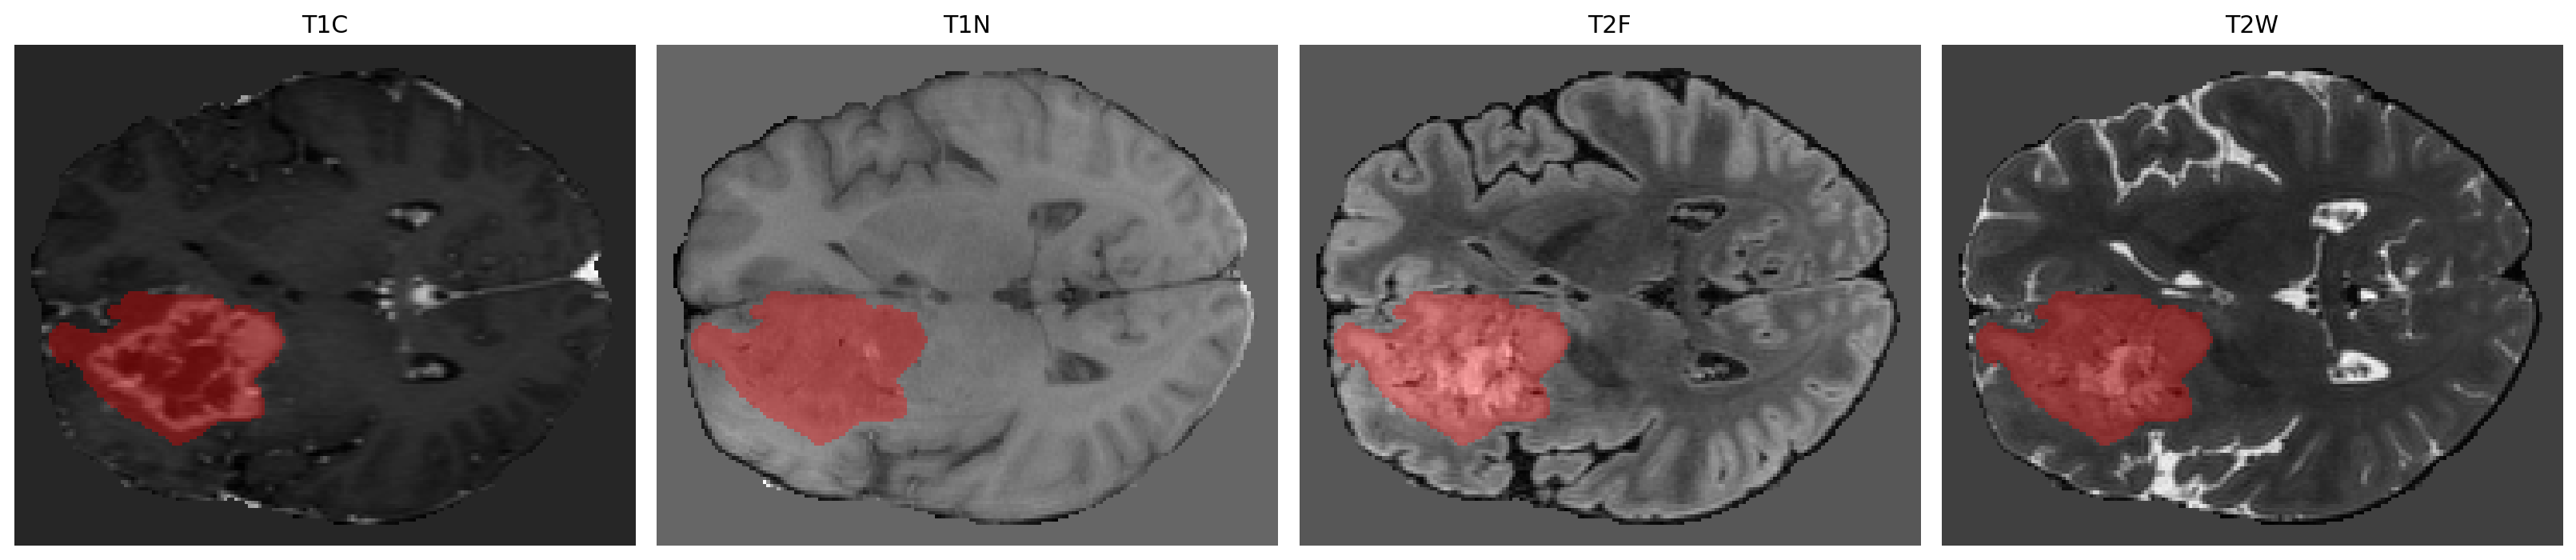
\includegraphics[width=0.92\textwidth]{figures/task1_example.png}
  \\\vspace{0.3cm}
  Best ET contrast modality in the executed analysis: \textbf{T1C}
\end{frame}

\begin{frame}{Models}
  \begin{itemize}
    \item Baseline: 2D U-Net.
    \item Upgrade: Attention U-Net.
    \item Loss: Dice + BCE.
    \item Augmentation: flips, rotations, scaling, Gaussian noise.
    \item Metrics: Dice for WT/TC/ET and HD95.
  \end{itemize}
\end{frame}

\begin{frame}{Baseline Training Artifact}
  \centering
  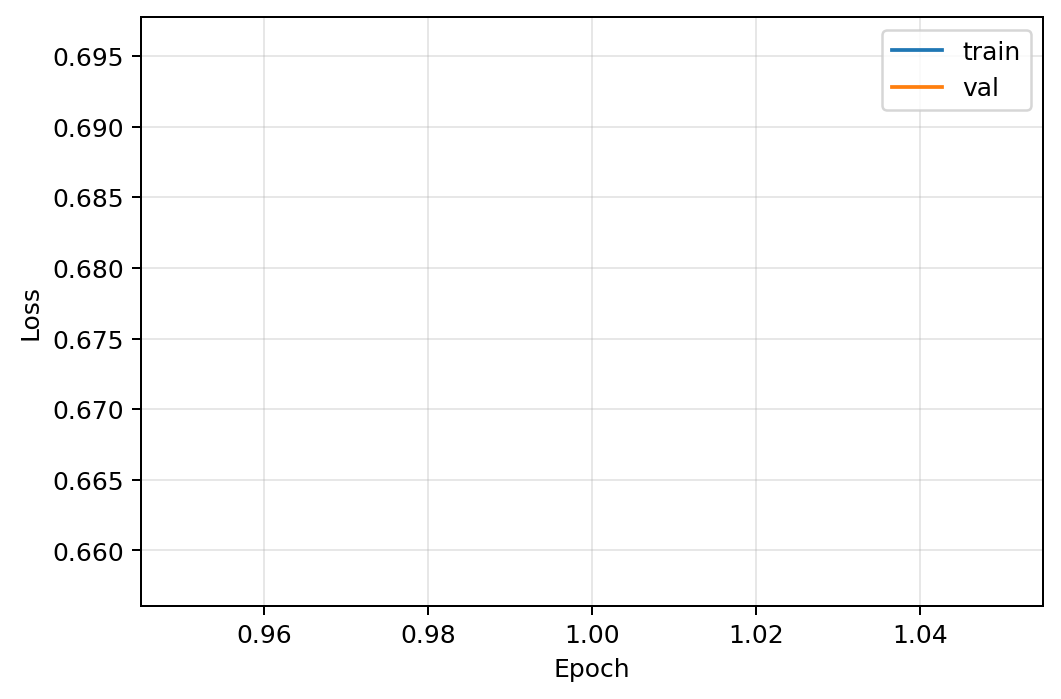
\includegraphics[width=0.78\textwidth]{figures/baseline_loss_curve.png}
\end{frame}

\begin{frame}{Experiment Comparison}
  \centering
  \begin{tabular}{lccc}
    \toprule
    Region & Baseline & Attention & $\Delta$ \\
    \midrule
    WT & 0.7063 & 0.6506 & -0.0557 \\
    TC & 0.5409 & 0.3834 & -0.1574 \\
    ET & 0.8008 & 0.6560 & -0.1448 \\
    \bottomrule
  \end{tabular}
  \\\vspace{0.4cm}
  In this verified smoke experiment, the baseline U-Net outperformed the attention variant.
\end{frame}

\begin{frame}{Worst-case Analysis}
  \begin{itemize}
    \item Hardest case in both models: \texttt{BraTS-GLI-00009-001}.
    \item Dominant failure reason: \textbf{small lesion size}.
    \item Other weak cases were linked mainly to low contrast.
  \end{itemize}
  \vspace{-0.2cm}
  \centering
  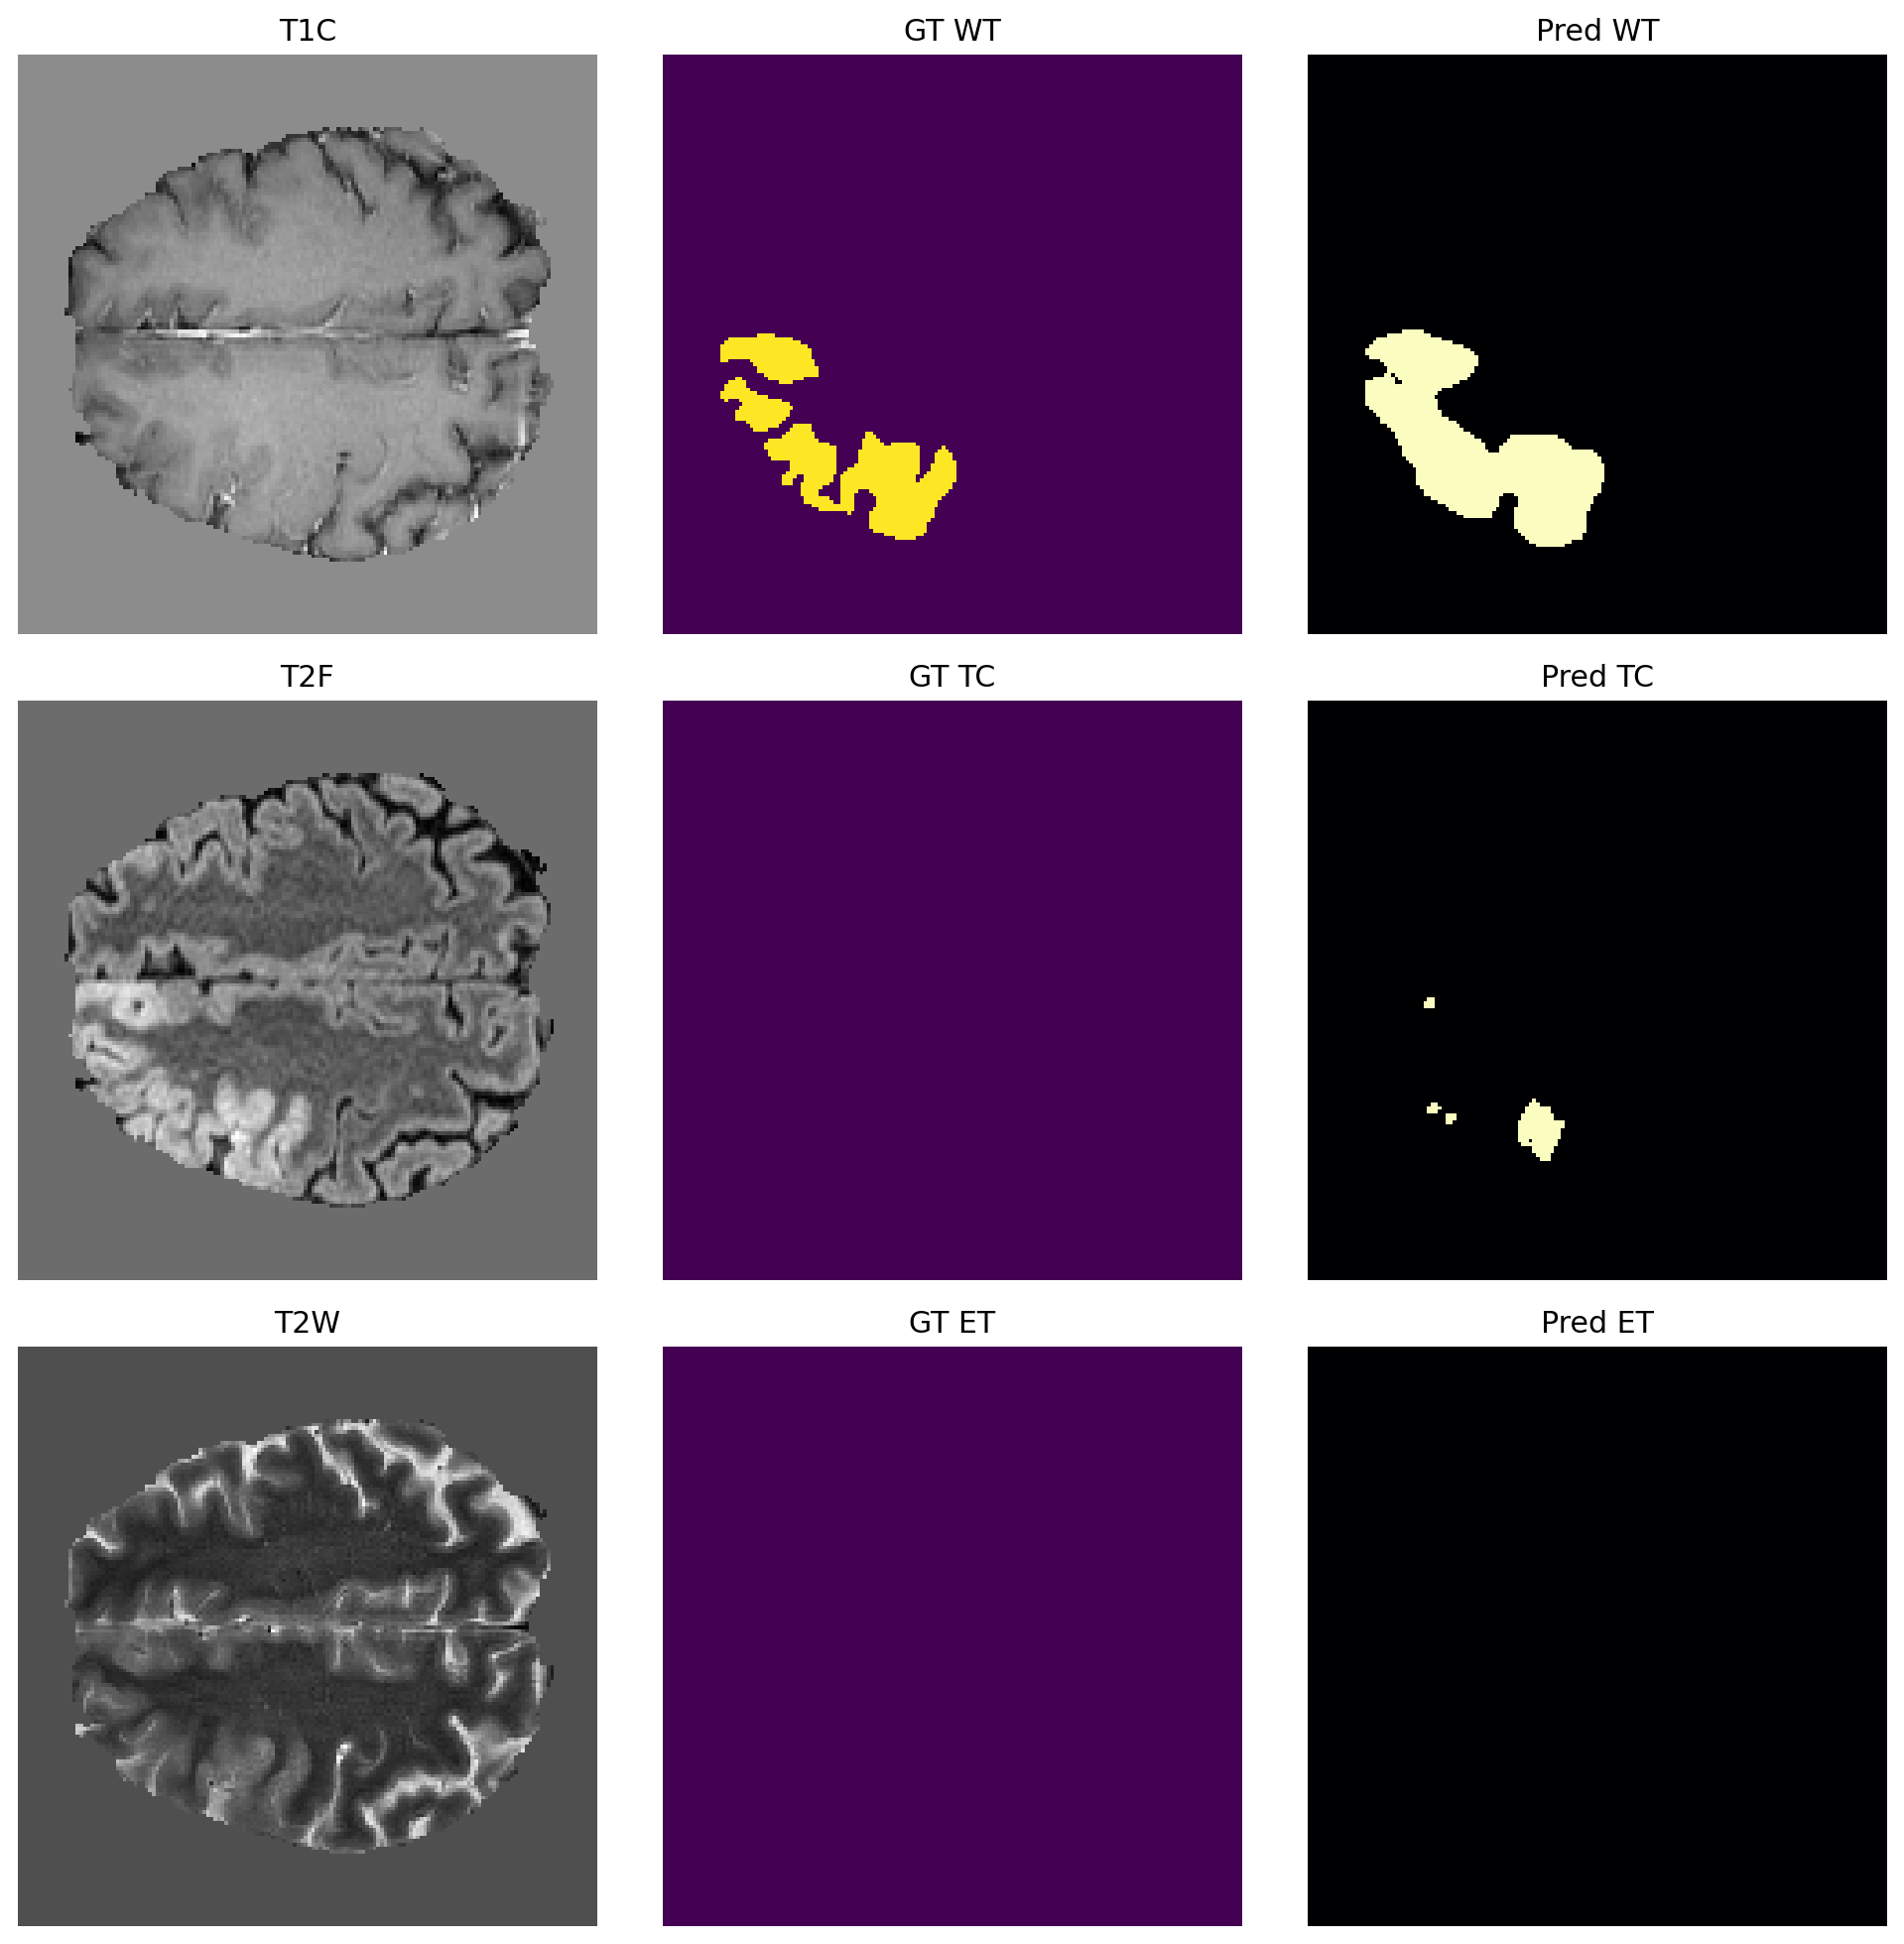
\includegraphics[width=0.52\textwidth]{figures/worst_case.png}
\end{frame}

\begin{frame}{Conclusion}
  \begin{itemize}
    \item Delivered a complete local BraTS coursework repository.
    \item Verified preprocessing, training, evaluation, and error-analysis scripts with real runs.
    \item The current outputs are smoke-scale but reproducible and ready for longer full training.
  \end{itemize}
\end{frame}

\end{document}
